\documentclass[aspectratio=169]{beamer}
\usepackage[utf8]{inputenc}
\usepackage[T1]{fontenc}
\usepackage{amsmath}
\usepackage{amsfonts}
\usepackage{amssymb}
\usepackage{graphicx}
\usepackage{tikz}
\usepackage{booktabs}
\usepackage{color}
\usepackage{multirow}
\usepackage[percent]{overpic}
\usetheme[
outer/progressbar=foot,
outer/numbering=none]{metropolis}

% theme settings
\metroset{titleformat=smallcaps}

% highlighting
\newcommand{\highlight}[2][yellow]{\mathchoice%
	{\colorbox{#1}{$\displaystyle#2$}}%
	{\colorbox{#1}{$\textstyle#2$}}%
	{\colorbox{#1}{$\scriptstyle#2$}}%
	{\colorbox{#1}{$\scriptscriptstyle#2$}}}%


% images
\graphicspath{ {D:/Users/saketh/Documents/GitHub/BECCS-Case-Study/code/matlab/simulation_april/}}

% sig stars
\def\sym#1{\ifmmode^{#1}\else\(^{#1}\)\fi}

\newcommand{\xoverbrace}[2][\vphantom{\dfrac{A}{A}}]{\overbrace{#1#2}}
\newcommand{\xunderbrace}[2][\vphantom{\dfrac{A}{A}}]{\underbrace{#1#2}}

\begin{document}
	\author{Saketh Aleti \& Gal Hochman}
	\title{Efficient Pollution Abatement in Electricity Markets with Intermittent Renewable Energy}
	%\subtitle{}
	%\logo{}
	\institute{Rutgers University}
	%\date{February 22}
	%\subject{}
	%\setbeamercovered{transparent}
	%\setbeamertemplate{navigation symbols}{}
\begin{frame}[plain]
	\maketitle
\end{frame}

%%%%% To do
%% Line up stuff between empirical methodology equations

\begin{frame}
\frametitle{Motivation}

\begin{block}{\centering Constructing a realistic model of intermittency}
\vspace{2em}
``\textit{\dots the economics of all generating technologies, both intermittent and dispatchable, can be evaluated based on the expected market value of the electricity that they will supply, their total life-cycle costs, and their associated expected profitability. Such an analysis would reflect the actual expected production profiles of dispatchable and intermittent technologies, the value of electricity supplied at different times, and other costs of intermittency associated with reliable network integration.}'' (Joskow, 2011)

\end{block}

\end{frame}



\begin{frame}
\frametitle{Motivation}
\vspace{1em}

\begin{block}{\centering Intermittency matters}
	
	\vspace{1em}
	\begin{overpic}[width=1\textwidth,tics=10]{../documents/exhibits/ercot_load.pdf} 
		\put (42,13) {\only<2>{$\Bigg\}$ Underproduction }}
		\put (71,37) {\only<2>{$\Big\}$ Overproduction }}
	\end{overpic}
	
\end{block}

\end{frame}


%%%%%%remove
\begin{frame}
\frametitle{Literature}

\begin{itemize}
	\setlength\itemsep{0.2em}
	\item Some literature approach the problem by numerically optimizing the capacity of intermittent renewables given reliability constraints\footnote{(Musgens \& Neuhoff, 2006), (Neuhoff et al., 2007)}
	\item Other papers study how intermittent technologies affect the market itself\footnote{(Ambec \& Crampes, 2012), (Chao, 2011), (Borenstein, 2012)}	
	\item A common top-down approach is to model intermittency through a CES function between different energy technologies\footnote{See Papageorgiou et al. (2017) for a survey of the literature taking this approach}
	%\item Consumers prefer to smooth their electricity consumption\footnote{(Schwarz et al., 2002), (Herriges et al., 1993), (King \& Shatrawka, 2011).}
	\item Our model is closest to Helm and Mier (2019)
\end{itemize}

\end{frame}


\begin{frame}
\frametitle{Model -- Overview}


\begin{figure}
	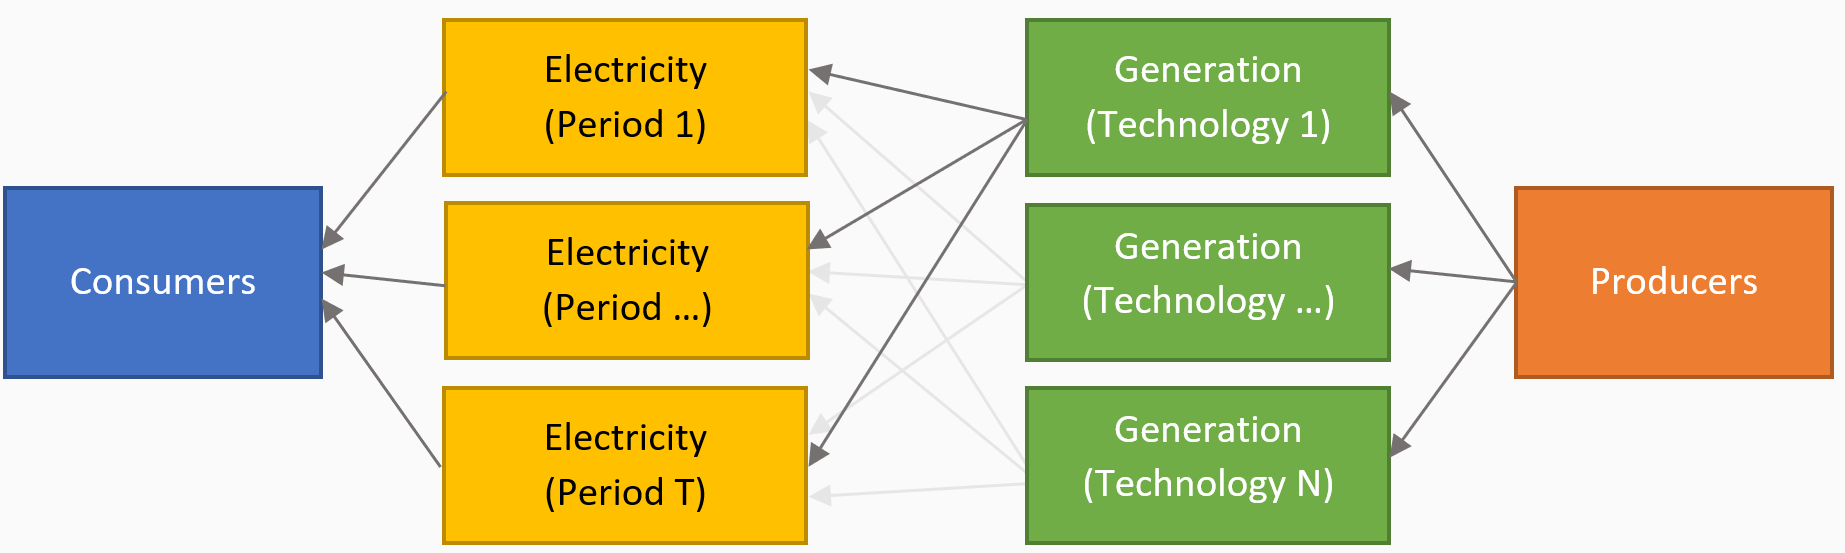
\includegraphics[width=0.8\textwidth]{../documents/exhibits/model_diagram.png} 
\end{figure}

\vspace{-1em}

\begin{itemize}
	\setlength\itemsep{0.2em}
	\item Multi-period model with electricity consumers and producers
	\item Consumers purchase electricity in each period to maximize utility
	\item Producers build up capacity in generation technologies to maximize profit
	\item Market reaches an equilibrium through variable electricity prices
\end{itemize}

\end{frame}

\begin{frame}
\frametitle{Model -- Overview}


\begin{figure}
	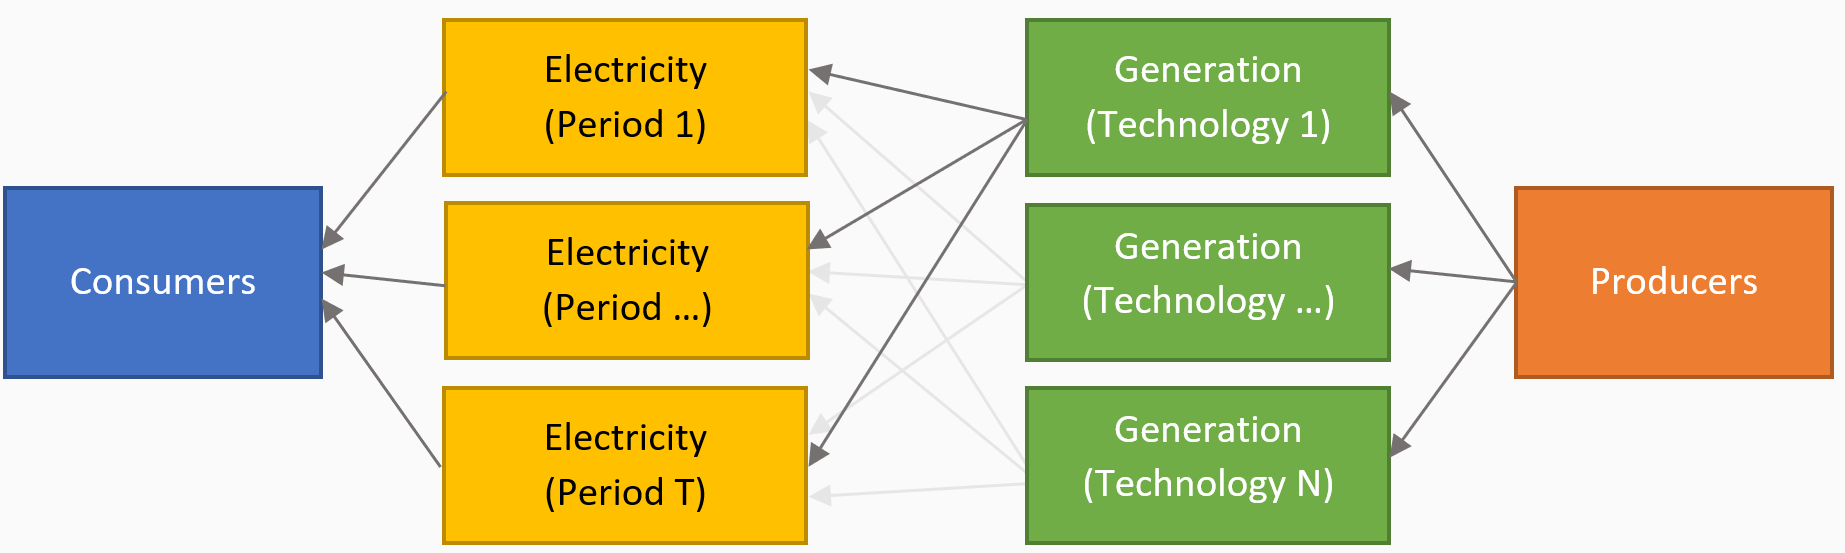
\includegraphics[width=0.8\textwidth]{../documents/exhibits/model_diagram.png} 
\end{figure}

\vspace{-0.8em}

\begin{itemize}
	\setlength\itemsep{0.2em}
	\item[$\implies$] Elasticity of substitution between renewables and fossil fuels is non-constant
	\item[$\implies$] The importance of intermittency (in terms of welfare) increases with the intermittency of present generation
	\item[$\implies$] Batteries can drastically increase the substitutability of renewables and fossil fuels
\end{itemize}

\end{frame}




\begin{frame}
\frametitle{Model -- Consumers}

%\begin{block}{Consumer assumptions}
%	\begin{itemize}
%		\setlength\itemsep{0.25em}
%		\item Representative consumer who purchases and uses electricity in each period
%		\item Consumers prefer to use different amounts of electricity at different times
%		\item Consumers will substitute electricity consumption across time periods based on relative prices\footnote{ This has been empirically studied by Schwarz et al. (2002), Herriges et al. (1993), King \& Shatrawka (2011).}
%	\end{itemize}
%\end{block}


\begin{columns}[T]%beamer
	
	\column{0.4\textwidth}
	\begin{figure}
		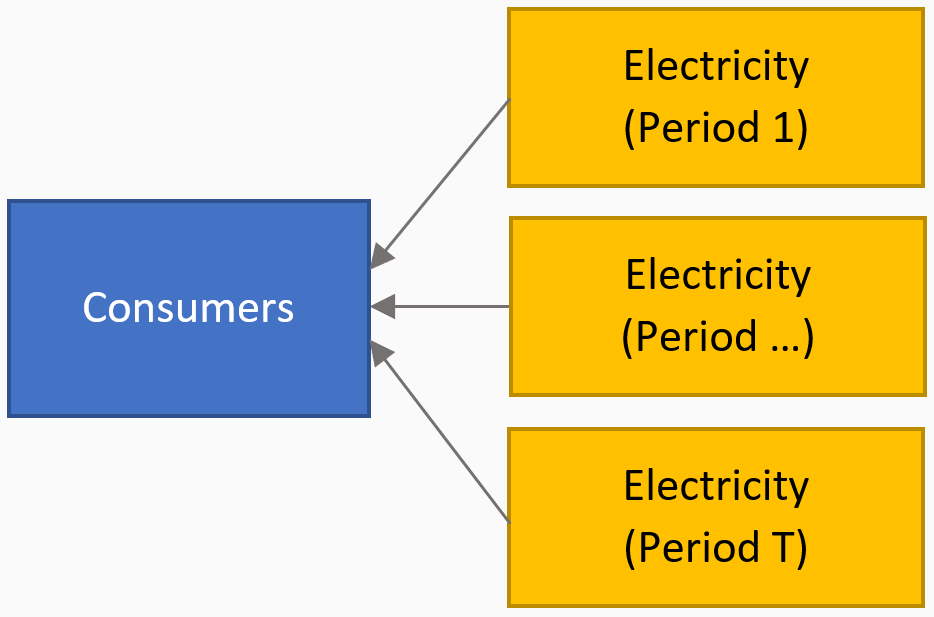
\includegraphics[width=1\textwidth]{../documents/exhibits/model_diagram_cons.png} 
	\end{figure}
	
	\column{0.6\textwidth}	
		\begin{block}{Consumer assumptions}
			\begin{itemize}
				\setlength\itemsep{0.25em}
				\item Representative consumer who purchases and uses electricity in each period
				\item Consumers prefer to use different amounts of electricity at different times
				\item Consumers will substitute electricity consumption across time periods based on relative prices%\footnote{ This has been empirically studied by Schwarz et al. (2002), Herriges et al. (1993), King \& Shatrawka (2011).}
			\end{itemize}
		\end{block}
	
\end{columns}


\end{frame}


\begin{frame}
\frametitle{Model -- Consumers}

\metroset{block=fill}

\vspace{1em}
\begin{block}{\centering{Consumer's Optimization Problem}}
	\small
	\begin{align*}
	\\[-3em] \text{\textbf{Utility}: } &U = \left( \sum_t \alpha_t Z_t^\phi  \right)^{1/\phi} \\[1em]
	\text{\textbf{Budget Constraint}: } &I = \sum_t p_t Z_t \\[-2.5em]
	\end{align*}
\end{block}

\begin{itemize}
	\setlength\itemsep{0.25em}
	\small
	\item $\alpha_t$ captures preference to use different amounts of electricity at different times
	\item $\phi$ captures preference to substitute electricity consumption across time periods based on relative prices
	\item  $\sigma = 1/(1-\phi)$ is the intertemporal elasticity of substitution for electricity consumption
	\item Total cost of electricity equals the cost of electricity consumed in each period
\end{itemize}

\end{frame}



\begin{frame}
\frametitle{Model -- Firms}


\begin{columns}[T]%beamer
	
	\column{0.4\textwidth}
	\begin{figure}
		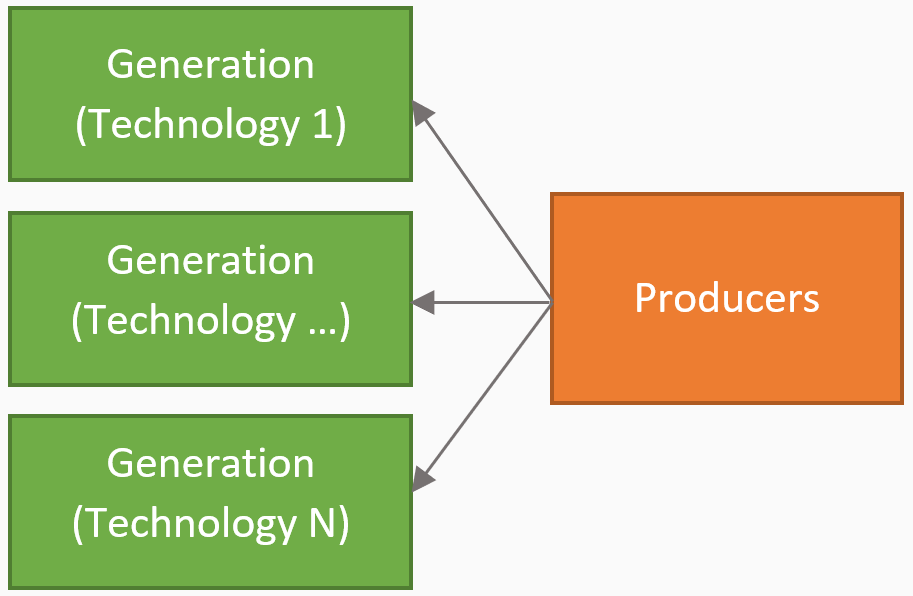
\includegraphics[width=1\textwidth]{../documents/exhibits/model_diagram_prod.png} 
	\end{figure}
	
	\column{0.6\textwidth}	
	\begin{block}{Producer assumptions}
		\begin{itemize}
			\setlength\itemsep{0.25em}
			\item Representative firm that maximizes profit
			\item Firms build a fixed amount of capacity in different generation technologies
			\item Different technologies can access different fractions of their capacity in each period
			\item Output is not stochastic; we focus our model on intermittency rather than reliability
		\end{itemize}
	\end{block}
		
\end{columns}




\end{frame}

\begin{frame}
\frametitle{Model -- Firms}

\metroset{block=fill}

\vspace{1em}
\begin{block}{\centering{Firm's Optimization Problem}}
	\small
	\begin{align*}
	\\[-3em] \text{\textbf{Profit}: } &\Pi = p^T Z - c^T X \\[1em]
	&= p^T \xi X - c^T X \\[-2.5em]
	\end{align*}
\end{block}

\begin{itemize}
	\setlength\itemsep{0.25em}
	\item Firms choose fixed quantities $X_i$ of each generation technology $i$ 
	\item Technology $i$ produces $\xi_{i,t}$ electricity per unit in period $t$
	\item Cost of building  $X_i$ units of generation technology $i$ is  $c_i X_i$
	\item Reminiscent of Joskow (2011) $\implies$ $X$ is chosen  ``\textit{\dots based on the expected market value of the electricity that they will supply, their total life-cycle costs, and their associated expected profitability\dots}''
\end{itemize}

\end{frame}

\begin{frame}
\frametitle{Model -- Solution}

\metroset{block=fill}

\begin{block}{\centering Equilibrium}
	\begin{align*}
	\\[-3em] \text{\textbf{Utility Max}: } Z_t &= \left(\frac{\alpha_t}{p_t} \right)^\sigma \frac{I}{\sum_t \alpha_t^\sigma p_t^{1-\sigma}} \\[1em]
	 \text{\textbf{Profit Max}: \hspace{0.1em} }	p &= \xi^{-1} c \\[-2.5em]
	\end{align*}
\end{block}

\vspace{1em}

\begin{itemize}
	\setlength\itemsep{0.25em}
	\item Consumer's optimum is the standard CES solution
	\item Analytically tractable only when $\sigma = 1$ and number of generation technologies equals the number of periods
	\item Can study the solution numerically by parametrizing $\xi, c, \alpha$, and $\sigma$. 
\end{itemize}


\end{frame}

\begin{frame}
\frametitle{Empirical Methodology}

\vspace{2em}
\begin{block}{\centering{Goal}}
	\centering \vspace{0.2em}
	Estimate the intertemporal elasticity of \\
	substitution for electricity consumption $\sigma$
\end{block}
\vspace{1em}

\begin{itemize}
	\setlength\itemsep{0.75em}
	\item <1->CES First order condition: $\dfrac{Z_t}{Z_s} = \left(\dfrac{\alpha_t \, p_s}{\alpha_s \, p_t} \right)^\sigma $
	\item <1->Cet par, an IES Of $\sigma$ implies a 1\% increase in the relative price of electricity $(P_{t}/P_{t+1})$  decreases relative electricity consumption $(Z_{t}/Z_{t+1})$  by $\sigma\%$
	\item <2->Directly affects the economic importance of intermittency
	\item <2->Literature has estimated $\sigma$ to be around 0.05 
\end{itemize}
\vspace{2.75em}

\end{frame}


\begin{frame}
\frametitle{Empirical Methodology -- Theory}



$$\xoverbrace{\ln (Z_{ t, i} / Z_{ s, i}) = -\sigma \ln (P_{t,i} / P_{s,i})}^{\text{CES First Order Condition}}$$
\vspace{-1.75em}
$$+  \sigma \ln (\alpha_{t,i} / \alpha_{s,i}) + u_i$$
\vspace{1em}
\begin{itemize}
	\setlength\itemsep{0.25em}
	\item $\sigma$ = Intertemporal elasticity of substitution for electricity consumption
	\item $\ln (Z_{t, i} / Z_{s, i})$ = Log Difference in electricity consumption
	\item $\ln (P_{t,i} / P_{s,i})$ = Log Difference in electricity prices
	\item $\alpha_{t,i},\, \alpha_{s,i}$ = Demand shifters
	\item Subscripts $t$ and $s$ refer to time periods while $i$ refers to observations
\end{itemize}
\vspace{2.75em}

\end{frame}



\begin{frame}
\frametitle{Empirical Methodology -- Theory}


	
	$$\xoverbrace{\ln (Z_{ t, i} / Z_{ s, i}) = -\sigma \ln (P_{t,i} / P_{s,i})}^{\text{CES First Order Condition}}$$
	\vspace{-1.5em}
	$$+  \xunderbrace{\,\gamma_{t,i}  CDD_{t,i} + \omega_{t,i} HDD_{t,i} + \gamma_{s,i} CDD_{s,i} +  \omega_{s,i} HDD_{s,i}  + \eta \Delta_{t,s}}_{\text{Demand Controls}} + u_i$$
	 
	\begin{itemize}
		\setlength\itemsep{0.25em}
		\item $\sigma$ = Intertemporal elasticity of substitution for electricity consumption
		\item $\ln (Z_{t, i} / Z_{s, i})$ = Log Difference in electricity consumption
		\item $\ln (P_{t,i} / P_{s,i})$ = Log Difference in electricity prices
		\item $CDD_{t,i}$ = Cooling Degree Days
		\item $HDD_{t,i}$ = Heating Degree Days
		\item $\Delta_{t,s}$ = Difference in months between periods $t$ and $s$
	\end{itemize}

\end{frame}


\begin{frame}
\frametitle{Empirical Methodology -- Theory}

\vspace{2em}
\begin{block}{\centering What if there was intertemporal substitution on the supply side?}
	
	\vspace{2em}
	\begin{itemize}
		\item During the 1973 oil crisis,  refineries increased gasoline stocks expecting higher future prices
		\item Previous literature has not accounted for endogeneity
		\item Might bias $\sigma$ downwards
	\end{itemize}
	
\end{block}



\end{frame}


\begin{frame}
\frametitle{Empirical Methodology -- Theory}

\vspace{1em}

\begin{table}
	\begin{tabular}{@{\extracolsep{2em}}lc}
		\multirow{2}{*}{\textbf{Demand:}}\quad & $\ln (Z_{ t, i} / Z_{ s, i}) = -\sigma \ln (P_{t,i} / P_{s,i}) + \,\gamma_{t,i}  CDD_{t,i} $\\
		& $+ \,\omega_{t,i} HDD_{t,i} + \gamma_{s,i} CDD_{s,i} +  \omega_{s,i} HDD_{s,i}  + \eta \Delta_{t,s} + u_i$ \\[1em]
		\multirow{2}{*}{\textbf{Supply:}}\quad & $\ln (Z_{ t, i} / Z_{ s, i}) = \beta \ln (P_{t,i} / P_{s,i})$\\
		& $+ \,\psi$  \hspace{-0.25em}\colorbox{yellow}{$\ln (C_{t,i} / C_{s,i})$}$  + v_{i}$
	\end{tabular}
\end{table}

\vspace{1em}

\begin{itemize}
	\item $\ln (C_{t,i} / C_{s,i})$ = Log Difference in coal prices
	\item Coal prices affect the supply of electricity but not its demand
	\item Can use IV to handle endogeneity
\end{itemize}


\end{frame}




\begin{frame}
\frametitle{Empirical Methodology -- Approach}


\begin{itemize}
	\setlength\itemsep{1em}
	\item Approach the problem using OLS, IV (2SLS), and a semiparametric regression
	\item \textbf{Semiparametric regression} - Partially Linear IV
	\begin{itemize}
		\item<1-> Places controls (degree days, time) and instrument (coal prices) in smooth, unknown functions estimated using Kernel regressions
		\item<2->  Error term assumed to be mean zero but may be non-Gaussian
		\item<3->  Will produce different results than 2SLS if these functions are \textit{actually} non-linear 
		\item<4->  I find semiparametric results are significantly different from 2SLS
	\end{itemize} 
\end{itemize}

\vspace{7.5em}

\end{frame}



\begin{frame}
\frametitle{Empirical Methodology -- Approach}

\vspace{0.1em}

\begin{itemize}
	\setlength\itemsep{1em}
	\item Approach the problem using OLS, IV (2SLS), and a semiparametric regression
	\item \textbf{Semiparametric regression} - Partially Linear IV
	\begin{itemize}
		\item Places controls (degree days, time) and instrument (coal prices) in smooth, unknown functions estimated using Kernel regressions
		\item Error term assumed to be mean zero but may be non-Gaussian
		\item Will produce different results than 2SLS if these functions are \textit{actually} non-linear 
		\item I find semiparametric results are significantly different from 2SLS
	\end{itemize} 
\end{itemize}

\begin{table}
	\begin{tabular}{@{\extracolsep{2em}}lc}
		\multirow{2}{*}{\textbf{Demand:}}\quad & $\ln (Z_{ t, i} / Z_{ s, i}) = -\sigma \ln (P_{t,i} / P_{s,i})   $ \\
		& $+ $ \colorbox{yellow}{$f(CDD_{t,i}, HDD_{t,i}, CDD_{s,i} , HDD_{s,i}, \Delta_{t,s} )$}$ + u_i$ \\[1em]
		\multirow{2}{*}{\textbf{Supply:}}\quad & $\ln (Z_{ t, i} / Z_{ s, i}) = \beta \ln (P_{t,i} / P_{s,i})$\\
		& $+ $\colorbox{yellow}{$g(\ln (C_{t,i} / C_{s,i}))$}$  + v_{i}$
	\end{tabular}
\end{table}


\end{frame}





\begin{frame}
\frametitle{Data}


\begin{itemize}
	\setlength\itemsep{1em}
	\item Panel consists of monthly data for each state in the US from 2011 to 2018
	\item Monthly retail electricity price and consumption data is obtained from the EIA
	\item Coal prices for the same period are also obtained from the EIA
	\item Degree day data is collected from the NOAA
	\item Each variable is trimmed by 1\%
\end{itemize}


\end{frame}






\begin{frame}
\frametitle{Results}


\begin{table}
\caption{Partially Linear IV Regression Results}
\label{table:3} 
\small
\begin{tabular}{@{\extracolsep{4em}}lccc} 
	\\[-5ex]\hline  
	\hline \\[-1.8ex] 
	& \multicolumn{3}{c}{\textit{Instrument: $ \ln (C_{t,i} / C_{s,i})$}} \\ 
	\cline{2-4} 
	%\\[-1.8ex] & ln\_load\_rel \textasciitilde ln\_price\_rel & ln\_load\_rel \textasciitilde (CDD\_1) & ln\_load\_rel \textasciitilde time\_diff + (CDD\_1) \\ 
	\\[-1.8ex] & (1) & (2) & (3)\\ [0.5ex]
	\hline \\[-1.8ex] 
	$\hat{\sigma} $ & 2.9976$^{***}$ & 1.2123$^{***}$ & \colorbox{yellow}{0.8847}$^{***}$ \\ 
	& (0.169) & (0.052) & (0.044) \\ [0.9ex]
	\hline \\[-1.8ex] 
	Time Control &   &   & Yes  \\ 
	Degree Day Controls &   & Yes  & Yes  \\ 
	Observations & 6817 & 6817 & 6817 \\
	\hline 
	\hline \\[-2.5ex] 
	\multicolumn{4}{@{}p{37em}@{}}{\scriptsize \textit{Note: } The log difference in coal price between period $t$ and $s$, $ \ln (C_{t,i} / C_{s,i})$, is used as an instrument in these regressions. The sample covers all 50 US states from 2011 to 2018; outliers are removed by trimming 1\% of each variable except $\Delta_{t,s}$. The unit of observation is a set $(t,s,i)$ where $t \neq s$ are months and $i$ is a state.  Robust standard errors are reported in parentheses. *p$\textless$0.05, **p$\textless$0.01, ***p$\textless$0.001}  \\ 
\end{tabular} 
\end{table}

\end{frame}


\begin{frame}
\frametitle{Discussion}

\vspace{2em}

\begin{block}{\centering What are the practical implications of IES $\boldsymbol{\sigma}$ = 0.88?}
\end{block}

\vspace{1em}

\begin{itemize}
	\setlength\itemsep{0.5em}
	\item<1-> Consider our model in a setting with two periods (peak and off-peak) and two technologies (solar and coal)
	\item<2-> We parametrize our  model using data on cost and efficiency from the EIA
	\item<3-> We numerically evaluate this model to understand the effects of intermittency
\end{itemize}

\end{frame}


\begin{frame}
\frametitle{Discussion}

\vspace{2em}

\begin{block}{Does intermittency motivate a CES relationship between renewables and fossil fuel technologies? }
	\begin{itemize}
		\setlength\itemsep{0.5em}
		\item<1-> Many papers assume electricity should be modeled as a CES function of renewable and fossil fuel capacity or capital
		\item<1-> Often something like: $Electricity = (\alpha \cdot {Renewables}^\phi + \beta \cdot {Fossils}^\phi)^{1/\phi}$
		\item<2-> Does this relationship arise in our model? Is the elasticity of substitution ($e$) between these technologies constant? 
		\item<2-> We numerically estimate the elasticity of substitution $e$ between solar and coal in our model
	\end{itemize}
\end{block}

\vspace{1em}

\end{frame}



\begin{frame}
\frametitle{Discussion}

\begin{block}{\centering The elasticity of substitution between technologies is not constant}
\end{block}

\hspace*{-1.5em}
\begin{overpic}[width=1.1\textwidth,tics=10]{../code/matlab/simulation_april/fig_elasticity_x.png} 
	\put (24,11.5) {\colorbox{yellow}{$\leftarrow$ More reliance on solar, lower $e$}}
	\put (46,36) {\colorbox{yellow}{More reliance on coal, higher $e$ $\rightarrow$ }}
\end{overpic}

\end{frame}




\begin{frame}
\frametitle{Discussion}

\begin{block}{\centering The elasticity of substitution between technologies is not constant}
\end{block}

\hspace*{-1.5em}
\begin{overpic}[width=1.1\textwidth,tics=10]{../code/matlab/simulation_april/fig_elasticity_x.png} 
	\put (20,33) {\colorbox{yellow}{\parbox{22em}{As the electricity supply becomes more intermittent, baseload technologies become more valuable}}}
\end{overpic}

\end{frame}

\begin{frame}
\frametitle{Discussion}

\begin{block}{\centering Demand for base load capacity becomes more inelastic with its price }
\end{block}

\hspace*{-1.5em}
\begin{overpic}[width=1.1\textwidth,tics=10]{../code/matlab/simulation_april/fig_coal_elas_x.png} 
	\put (35,22) {\colorbox{yellow}{\parbox{22em}{As the electricity supply becomes more intermittent, baseload technologies become more valuable}}}
\end{overpic}

\end{frame}


\begin{frame}
\frametitle{Discussion}

\begin{block}{Why does a non-linear elasticity of substitution between intermittent and base load technologies matter?}
	\begin{itemize}
		\setlength\itemsep{0.5em}
		\item Over time, we may expect the share of renewable energy to increase $\implies$ elasticity of substitution between renewables and fossil fuels will decrease over time
		\item Taxes/subsidies need to be increasingly larger to shift the same fraction of capacity towards renewables and away from fossil fuels 
		\item Models assuming a constant elasticity of substitution may not be realistic
	\end{itemize}
\end{block}
\end{frame}


\begin{frame}
\frametitle{Discussion}

\begin{block}{How should we handle pollution abatement when generation is intermittent?}
	\begin{itemize}
		\setlength\itemsep{0.5em}
		\item<1-> Carbon taxes still work
		\item<2-> Should also account for its distributional effects
		\item<3-> Greater welfare losses in regions without access to non-intermittent renewables
		\item<4-> Can turn into an equity--efficiency trade--off
	\end{itemize}
\end{block}
\end{frame}


\begin{frame}
\frametitle{Discussion}

\begin{block}{\centering Distribution of Hydrothermal and Geothermal Plants (EIA, 2019)}
\end{block}

\begin{figure}
	\vspace{-1em}
	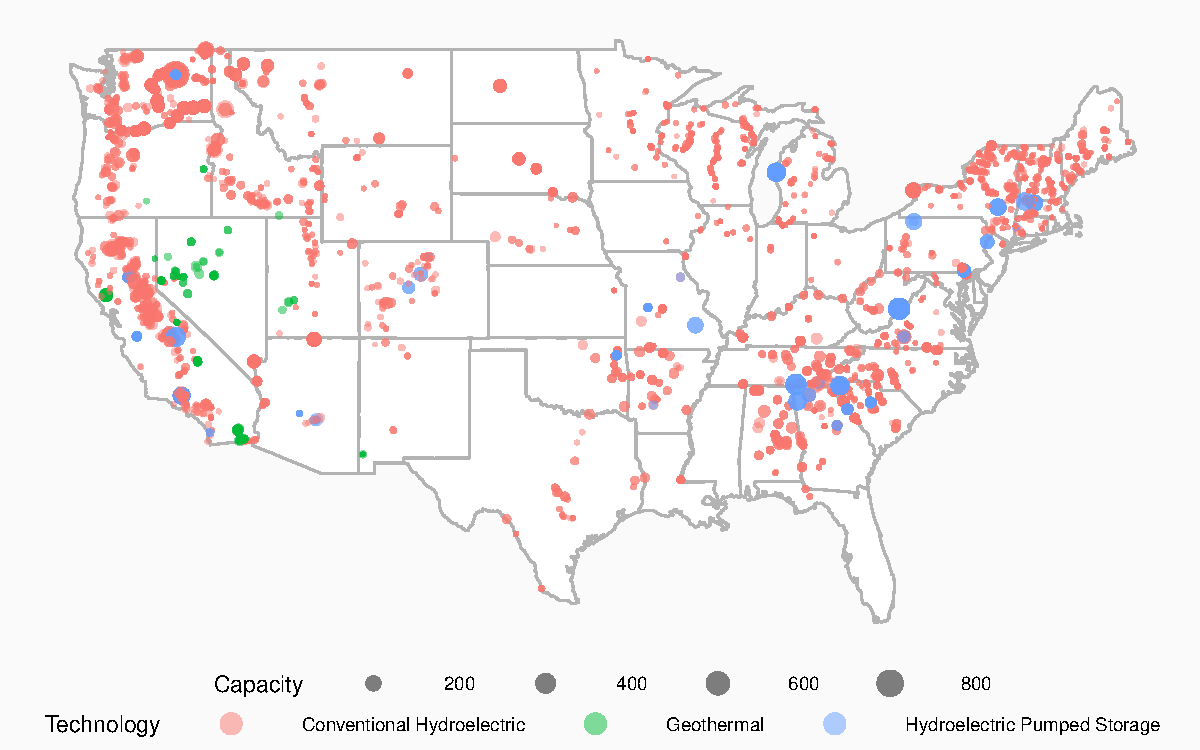
\includegraphics[width=0.8\textwidth]{../documents/exhibits/rel_renew_map.pdf} 
\end{figure}

\end{frame}

\begin{frame}
\frametitle{Discussion -- Batteries}

\begin{block}{Improving battery technology can make a significant difference}
	\begin{itemize}
		\setlength\itemsep{0.5em}
		\item Reducing the intermittency of renewables greatly increases their substitutability
		\item Mitigates the distributional side effects of intermittency + carbon taxes
		\item Can roughly approximate the effects of batteries in our model by shifting solar output to the off-peak period when it under-produces
	\end{itemize}
\end{block}
\end{frame}



\begin{frame}
\frametitle{Discussion -- Batteries}

\begin{block}{\centering Using batteries to shift solar output greatly increases its substitutability}
\end{block}

\hspace*{-1.5em}
\begin{overpic}[width=1.1\textwidth,tics=10]{../code/matlab/simulation_april/fig_batteries_x.png} 
	\put (31,30) {\colorbox{yellow}{\parbox{15em}{Shifting 10\% of solar output doubles the elasticity when the majority of generation is intermittent}}}
	\linethickness{2pt}
	\put(31,27){\color{black}\vector(-1,-1){6.5}}
\end{overpic}

\end{frame}


\begin{frame}
\frametitle{Discussion -- Batteries}

\begin{block}{\centering Initially, increasing returns to batteries and substitutability}
\end{block}

\hspace*{-1.5em}
\begin{overpic}[width=1.1\textwidth,tics=10]{../code/matlab/simulation_april/fig_batteries_x.png} 
	\put (32,35) {\colorbox{yellow}{\parbox{16em}{Elasticity increases by $\approx 25\%$ for a 5\% shift but by $\approx 70\%$ for a 10\% shift}}}
	\linethickness{2pt}
	\put(70,31.5){\color{black}\vector(4,-3){8}}
	\put(73,31.5){\color{black}\vector(3,-2){3}}
\end{overpic}

\end{frame}

\begin{frame}
\frametitle{Discussion -- Improving Models}

\begin{block}{How can future models of energy generation substitutability be improved?}
	\begin{itemize}
		\setlength\itemsep{0.5em}
		\item <1-> Assuming a constant elasticity of substitution between renewables and fossil fuels does not accurately capture intermittency
		\item <1-> Empirical estimates of the elasticity of substitution may be incorrect since the functional form (CES) does not seem to be appropriate 
		\item <2-> Directly implementing our model may not allow for analytical tractability
		\item <2-> Can try the variable elasticity of substitution (VES) form instead\footnote{The VES function was first defined in Revankar (1971).}
	\end{itemize}
\end{block}
\end{frame}


\begin{frame}
\frametitle{Discussion -- Improving Models}

\begin{block}{\centering VES approximation of the relationship between solar and coal}
\end{block}

\hspace*{-1.5em}
\begin{overpic}[width=1.1\textwidth,tics=10]{../code/matlab/simulation_april/fig_ves_approx_x.png} 
\end{overpic}

\end{frame}


\begin{frame}
\frametitle{Discussion -- Improving Models}

\begin{block}{What exactly is the VES function?}
	\begin{itemize}
		\setlength\itemsep{0.5em}
		\item Assumes that the elasticity of substitution between factors varies as a linear function of their quantities
		\item Can be empirically estimated
		\item Simpler to implement in a theoretical or numerical framework than our model
	\end{itemize}
	\begin{align*}
	&Z = \gamma X_1^{\omega(1-\delta \rho)} \left( X_2 + (\rho - 1) X_1 \right)^{\omega \delta \rho} \\
	&\highlight{e = 1 + \beta (X_1 / X_2)} \\
	&\,\beta = (\rho - 1) / ( 1- \delta \rho ) 
	\end{align*}
	\vspace{-4ex}
	$$\gamma > 0, \quad \omega > 0, \quad0 < \delta < 1, \quad 0 \leq \delta \rho \leq 1 , \quad (X_2/X_1) >  -\beta $$
\end{block}

\end{frame}

\begin{frame}
\frametitle{Conclusion}

\begin{itemize}
	\setlength\itemsep{0.75em}
	\item Welfare effects of carbon taxes and renewable subsidies depend on the intermittency of renewables and thus vary geographically
	\item Intermittency can create a trade-off between efficiently and equitably preventing climate change
	\item Subsidizing battery research can complement other policies by increasing the substitutability of renewable and fossil energy while mitigating their unintentional distributional consequences 
	\item The VES function can do a reasonable job of approximating the substitutability between renewables and fossil fuels
\end{itemize}

\end{frame}


%%%%%%% References
\begin{frame}[allowframebreaks]
\frametitle{References}
\tiny 

\begin{itemize}
	
\item Acemoglu, D., Aghion, P., Bursztyn, L., \& Hemous, D. (2012). The Environment and Directed Technical Change. American Economic Review, 102(1), 131–166. https://doi.org/10.1257/aer.102.1.131

\item Adelman, M. A. (1995). The genie out of the bottle: World oil since 1970. MIT Press.

\item Ambec, S., \& Crampes, C. (2012). Electricity provision with intermittent sources of energy. Resource and Energy Economics, 34(3), 319–336. https://doi.org/10.1016/j.reseneeco.2012.01.001

\item Aubin, C., Fougere, D., Husson, E., \& Ivaldi, M. (1995). Real-time pricing of electricity for residential customers: Econometric analysis of an experiment. Journal Of Applied Econometrics, 10, S171–S191.

\item Borenstein, S. (2012). The Private and Public Economics of Renewable Electricity Generation. Journal of Economic Perspectives, 26(1), 67–92. https://doi.org/10.1257/jep.26.1.67

\item Chao, H. (2011). Efficient pricing and investment in electricity markets with intermittent resources. Energy Policy, 39(7), 3945–3953. https://doi.org/10.1016/j.enpol.2011.01.010

\item Climate Prediction Center (2019). Degree Days Statistics. National Oceanic and Atmospheric Administration. https://www.cpc.ncep.noaa.gov/products/analysis\_monitoring/cdus/degree\_days/

\item Delarue, E., De Jonghe, C., Belmans, R., \& D’Haeseleer, W. (2010). Applying portfolio theory to the electricity sector: Energy versus power. Energy Economics, 33(1), 12–23. https://doi.org/10.1016/j.eneco.2010.05.003

\item Deryugina, T., Mackay, A., \& Reif, J. (2017). The Long-Run Dynamics of Electricity Demand: Evidence from Municipal Aggregation. NBER Working Paper Series. https://doi.org/10.3386/w23483

\item Electricity Information Administration (2019a). Net generation, United States, all sectors, annual. Electricity Data Browser. https://www.eia.gov/electricity/data/browser

\item Electricity Information Administration (2019b). Levelized Cost and Levelized Avoided Cost of New Generation. Annual Energy Outlook 2019. https://www.eia.gov/outlooks/aeo/pdf/electricity\_generation.pdf

\item Electricity Information Administration (2019c). U.S. renewable electricity generation has doubled since 2008. Today in Energy. https://www.eia.gov/todayinenergy/detail.php?id=38752

\item Fan, S., \& Hyndman, R. (2011). The price elasticity of electricity demand in South Australia. Energy Policy, 39(6), 3709–3719. https://doi.org/10.1016/j.enpol.2011.03.080

\item Foley, A., Leahy, P., Marvuglia, A., \& Mckeogh, E. (2012). Current methods and advances in forecasting of wind power generation. Renewable Energy, 37(1), 1–8. https://doi.org/10.1016/j.renene.2011.05.033

\item Geroski, P. (2000). Models of technology diffusion. Research Policy. Elsevier B.V. https://doi.org/10.1016/S0048-7333(99)00092-X

\item Helm, C., \& Mier, M. (2019). On the efficient market diffusion of intermittent renewable energies. Energy Economics, 80, 812–830. https://doi.org/10.1016/j.eneco.2019.01.017

\item Herriges, J., Baladi, S., Caves, D., \& Neenan, B. (1993). The Response of Industrial Customers to Electric Rates Based Upon Dynamic Marginal Costs. The Review of Economics and Statistics, 75(3), 446. https://doi.org/10.2307/2109458

\item Joskow, P. (2011). Comparing the Costs of Intermittent and Dispatchable Electricity Generating Technologies. American Economic Review, 101(3), 238–241. https://doi.org/10.1257/aer.101.3.238

\item King, Kathleen, and Peter Shatrawka (1994). "Customer Response to a Permanent Time- Varying
Pricing Program in the United Kingdom." Laurits R. Christensen Associates, Madison,
Wisconsin.

\item Mohajeryami, S., Moghaddam, I., Doostan, M., Vatani, B., \& Schwarz, P. (2016). A novel economic model for price-based demand response. Electric Power Systems Research, 135, 1–9. https://doi.org/10.1016/j.epsr.2016.03.026

\item Musgens, F., \& Neuhoff, K. (2006). Modelling Dynamic Constraints in Electricity Markets and the Costs of Uncertain Wind Output. Faculty of Economics.

\item Neuhoff, K., Cust, J. \& Keats, K. (2007). Implications of intermittency and transmission constraints for renewables deployment. Cambridge Working Papers in Economics 0711, Faculty of Economics, University of Cambridge.

\item Newey, W. (1990). Efficient Instrumental Variables Estimation of Non-linear Models. Econometrica, 58(4), 809–837. https://doi.org/10.2307/2938351

\item ORNL (2004). Measurement practices for reliability and power quality. A toolkit of reliability measurement practices. U.S. Department of Energy. https://info.ornl.gov/sites/publications/Files/Pub57467.pdf

\item Papageorgiou, C., Saarn, M., \& Schulte, P. (2017). Substitution between clean and dirty energy inputs: a macroeconomic perspective.(Author abstract). Review of Economics and Statistics, 99(2), 201–212. https://doi.org/10.1162/REST\_a\_00623

\item Reiss, P., \& White, M. (2005). Household Electricity Demand, Revisited. The Review of Economic Studies, 72(252), 853. Retrieved from http://search.proquest.com/docview/204335314/

\item Revankar, N. (1971). A Class of Variable Elasticity of Substitution Production Functions. Econometrica, 39(1), 61–71. https://doi.org/10.2307/1909140

\item Schwarz, P., Taylor, T., Birmingham, M., \& Dardan, S. (2002). Industrial response to electricity real-time prices: short run and long run. Economic Inquiry, 40(4), 597–610. https://doi.org/10.1093/ei/40.4.597

\item Shahriari, M., \& Blumsack, S. (2018). The capacity value of optimal wind and solar portfolios. Energy, 148, 992–1005. https://doi.org/10.1016/j.energy.2017.12.121

\item Silverman, B. (1986). Density estimation for statistics and data analysis. London; Chapman and Hall.

\item Zhou, S. \& Teng, F., (2013). Estimation of urban residential electricity demand in China using household survey data.(Statistical data). Energy Policy, 61, 394–402.

\item Staiger, D., \& Stock, J. (1997). Instrumental Variables Regression with Weak Instruments. Econometrica, 65(3), 557–586. https://doi.org/10.2307/2171753

\item U.S. Bureau of Economic Analysis (2019). Personal consumption expenditures: chain-type price index. FRED, Federal Reserve Bank of St. Louis. https://fred.stlouisfed.org/series/PCEPI, April 27, 2019.

\item Wolak, F., \& Patrick, R. (2001). The Impact of Market Rules and Market Structure on the Price Determination Process in the England and Wales Electricity Market. NBER Working Paper Series. https://doi.org/10.3386/w8248

\item Woo, C., Chow, P., \& Horowitz, I. (1996). Optional real-time pricing of electricity for industrial firms. Pacific Economic Review, 1(1), 79–92. https://doi.org/10.1111/j.1468-0106.1996.tb00175.x

\item Zarnikau, J. (1990). Customer Responsiveness to Real-Time Pricing of Electricity. The Energy Journal, 11(4), 99. https://doi.org/10.5547/ISSN0195-6574-EJ-Vol11-No4-6

\end{itemize}

\end{frame}

\begin{frame}
\frametitle{Appendix -- OLS Results}

\begin{table}[t] \centering 
	\caption{OLS Regression Results}
	\label{table:1} 
	\footnotesize
	\begin{tabular}{@{\extracolsep{5pt}}lcccccc} 
		\\[-5ex]\hline  
		\hline \\[-1.8ex] 
		& \multicolumn{6}{c}{\textit{Dependent variable:} $\ln (Z_{ t, i} / Z_{ s, i})$} \\ [0.5ex]
		\cline{2-7} 
		\\[-1.8ex] & (1) & (2) & (3) & (4) & (5) & (6)\\ [0.5ex]
		\hline \\[-1.8ex] 
		$-\ln (P_{t,i} / P_{s,i})$ & 0.937$^{***}$ & 1.075$^{***}$ & 1.098$^{***}$ & 1.074$^{***}$ & 1.263$^{***}$ & 1.305$^{***}$ \\ 
		& (0.030) & (0.026) & (0.026) & (0.224) & (0.172) & (0.169) \\  [0.9ex]
		\hline \\[-1.8ex] 
		Time Control &   &   & Yes &   &   & Yes  \\ 
		Degree Day Controls &   & Yes  & Yes &   & Yes  & Yes \\ 
		State FEs &   &   &   & Yes & Yes & Yes \\ 
		Observations & 6,817 & 6,817 & 6,817 & 6,817 & 6,817 & 6,817 \\ 
		Adjusted R$^{2}$ & 0.079 & 0.506 & 0.508 & 0.085 & 0.518 & 0.520 \\  
		F Statistic & 582$^{***}$  & 1399$^{***}$  & 1172$^{***}$ & 685$^{***}$  & 1474$^{***}$  & 1241$^{***}$  \\ [0.5ex]
		\hline 
		\hline \\[-1.8ex] 
		%\multicolumn{7}{@{}p{41.4em}@{}}{\textit{Note: } The sample covers all 50 US states from 2011 to 2018; outliers are removed by trimming 1\% of each variable except $\Delta_{t,s}$. The unit of observation is a set $(t,s,i)$ where $t \neq s$ are months and $i$ is a state. The coefficient on $-\ln (P_{t,i} / P_{s,i})$ is the estimate of $\sigma$. The variable $\Delta_{t,s}$ is the difference in months between periods $t$ and $s$. CDD$_t$ and HDD$_t$ refer to the total number of heating and cooling degree days in month $t$. We scale the coefficients on degree days for clarity. Robust standard errors are reported in parentheses. *p$\textless$0.05, **p$\textless$0.01, ***p$\textless$0.001}  \\ 
	\end{tabular} 
\end{table}

\end{frame}


\begin{frame}
\frametitle{Appendix -- IV Results}

\begin{table}[h] \centering 
	\caption{IV (2SLS) Regression Results}
	\label{table:2} 
	\scriptsize
	\begin{tabular}{@{\extracolsep{4pt}}lcccccc} 
		\\[-6ex]\hline  
		\hline \\[-1.6ex] 
		& \multicolumn{3}{c}{First-Stage} & \multicolumn{3}{c}{Second-Stage} \\ [0.5ex]
		& \multicolumn{3}{c}{\textit{Dep. Variable:} $\ln (P_{t,i} / P_{s,i})$ } & \multicolumn{3}{c}{\textit{Dep. Variable:}  $\ln (Z_{ t, i} / Z_{ s, i})$}\\ [0.5ex]
		\cmidrule(lr){2-4} \cmidrule(lr){5-7}\\[-2.9ex] 
		& (A.1) & (B.1) & (C.1) & (A.2) & (B.2) & (C.2)\\ [0.5ex]
		\hline \\[-1.8ex] 
		$ \ln (C_{t,i} / C_{s,i})$ & $-$0.042$^{***}$ & $-$0.018$^{***}$ & $-$0.018$^{***}$ &  &  &  \\ 
		& (0.002) & (0.002) & (0.002) &  &  &  \\ 
		& & & & & & \\[-1ex]
		$-\ln (P_{t,i} / P_{s,i})$ &  &  &  & 2.978$^{***}$ & 5.896$^{***}$ & 5.818$^{***}$ \\ 
		&  &  &  & (0.180) & (0.548) & (0.524) \\   [0.9ex]
		\hline \\[-1.8ex] 
		Time Control &   &   & Yes &   &   & Yes  \\ 
		Degree Day Controls &   & Yes  & Yes &   & Yes  & Yes \\ 
		State FEs &  Yes & Yes  & Yes  & Yes & Yes & Yes \\ 
		Observations & 6817 & 6817 & 6817 & 6817 & 6817 & 6817 \\ 
		Adjusted R$^{2}$ & 0.061 & 0.264 & 0.293 & &  &  \\ 
		F Statistic & 443$^{***}$  & 489$^{***}$ & 472$^{***}$  &  &  &  \\ 
		\hline 
		\hline \\[-1.8ex] 
		%\multicolumn{7}{@{}p{41.5em}@{}}{\textit{Note: } The log difference in coal price between period $t$ and $s$, $ \ln (C_{t,i} / C_{s,i})$, is used as an instrument in these regressions. The sample covers all 50 US states from 2011 to 2018; outliers are removed by trimming 1\% of each variable except $\Delta_{t,s}$. The unit of observation is a set $(t,s,i)$ where $t \neq s$ are months and $i$ is a state. The coefficient on $\ln (P_{t,i} / P_{s,i})$ is an estimate of $-\sigma$. The variable $\Delta_{t,s}$ is the difference in months between periods $t$ and $s$. CDD$_t$ and HDD$_t$ refer to the total number of heating and cooling degree days in month $t$. We scale the coefficients on degree days for clarity. Robust standard errors are reported in parentheses. *p$\textless$0.05, **p$\textless$0.01, ***p$\textless$0.001}  \\ 
	\end{tabular} 
\end{table}


\end{frame}





\begin{frame}
\frametitle{Appendix -- Model Parameters}

$$\underbrace{\alpha_t = 0.6, \,\alpha_s = 0.4}_{Demand\,\,parameters}, \,\underbrace{\xi_1 = (1, \, 1), \,\xi_2 = (1, \, 0.1)}_{Output\,\,parameters}, \,\underbrace{c_1 = 104.3, \,c_2 = 60}_{Cost \,\, parameters}$$

\begin{itemize}
	\setlength\itemsep{0.5em}
	\item We normalize quantity units in terms of capacity, so cost is given in \$/MWh and output is given as the fraction of capacity available in each period
	\item EIA LCOE estimates for 2023 for ``Coal with 30\% CCS'' and ``Solar PV''  are 104.3\$/MWh and 60\$/MWh $\implies$ $c_1 = 104.3$, $c_2 = 60$
	\item Based on the graph of ERCOT loads from earlier, consumers prefer that $\approx$ 60\% of their energy arrive between 900-2400 $\implies$ $(\alpha_t, \alpha_s) = (0.6, 0.4)$
	\item For same periods, solar output seems to be $\approx 10:1 \implies \xi_2 = (1, \, 0.1)$
	\item Coal output is assumed to be constant over both periods $\implies \xi_1 = (1, \, 1)$
\end{itemize}

\end{frame}

\end{document}